\subsection{Partitions, Congruence, and Quotients}

\begin{proposition} \label{prop:equivalence-relations-partitions} \hlt{Equivalence Classes Partition the Set}\\
Let $\sim$ be an equivalence relation on $X$. Then the equivalence classes form a partition of $X$.
\begin{proof}
Every $x\in X$ lies in $[x]$ since $x\sim x$. If $[x]\cap[y]\neq\emptyset$, choose $z$ in the intersection.\\
Then $x\sim z\sim y$, so $u\in[x]$ implies $u\sim y$ and $u\in[y]$. Hence $[x]\subseteq[y]$, and symmetry gives equality.\\
\hlt{Structural Commentary}: Equivalence means partition.\\
\hlt{Key Insight}: Touching classes coincide.
\end{proof}
\end{proposition}

\begin{figure}[H]
  \centering
  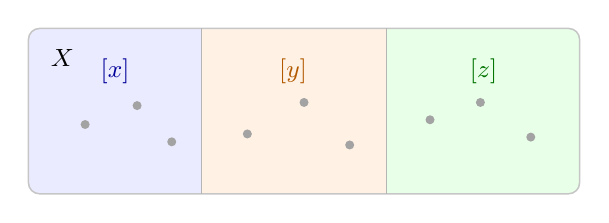
\begin{tikzpicture}[
  every node/.style={font=\small},
  ambient/.style={draw=gray!45, line width=0.55pt},
  seam/.style={draw=gray!58, line width=0.45pt},
  point/.style={circle, fill=gray!72, inner sep=1.15pt}
]
  \begin{scope}
    \clip[rounded corners=4pt] (0,0) rectangle (7.0,2.1);
    \fill[blue!8] (0,0) rectangle (2.2,2.1);
    \fill[orange!10] (2.2,0) rectangle (4.55,2.1);
    \fill[green!9] (4.55,0) rectangle (7.0,2.1);
  \end{scope}

  \draw[ambient, rounded corners=4pt] (0,0) rectangle (7.0,2.1);
  \draw[seam] (2.2,0) -- (2.2,2.1);
  \draw[seam] (4.55,0) -- (4.55,2.1);

  \node[anchor=north west] at (0.16,1.96) {$X$};
  \node[blue!60!black] at (1.10,1.55) {$[x]$};
  \node[orange!70!black] at (3.36,1.55) {$[y]$};
  \node[green!45!black] at (5.78,1.55) {$[z]$};

  \node[point] at (0.72,0.88) {};
  \node[point] at (1.38,1.12) {};
  \node[point] at (1.82,0.66) {};
  \node[point] at (2.78,0.76) {};
  \node[point] at (3.50,1.16) {};
  \node[point] at (4.08,0.62) {};
  \node[point] at (5.10,0.94) {};
  \node[point] at (5.74,1.16) {};
  \node[point] at (6.38,0.72) {};
\end{tikzpicture}

  \caption{Equivalence classes form disjoint blocks that cover the underlying set.}
  \label{fig:equivalence-classes-partition}
\end{figure}

\begin{proposition} \label{prop:partitions-determine-equivalence-relations} \hlt{Partitions Determine Equivalence Relations}\\
Let $\mathcal{F}$ be a partition of $X$. For $x\in X$, let $B_x\in\mathcal{F}$ be the unique block with $x\in B_x$.\\
Define a relation $\sim_{\mathcal{F}}$ on $X$ by $x\sim_{\mathcal{F}}y$ iff $B_x=B_y$.
\begin{enumerate}[label=(\roman*)]
\setlength{\itemsep}{0pt}
\item $\sim_{\mathcal{F}}$ is an equivalence relation on $X$.
\item For every $x\in X$, $[x]_{\sim_{\mathcal{F}}}=B_x$; hence the equivalence classes are exactly the members of $\mathcal{F}$.
\end{enumerate}
\begin{proof}
\begin{enumerate}[label=(\roman*)]
\setlength{\itemsep}{0pt}
\item For $x\in X$, $B_x=B_x$, so $x\sim_{\mathcal{F}}x$. If $x\sim_{\mathcal{F}}y$, then $B_x=B_y$, hence $B_y=B_x$ and $y\sim_{\mathcal{F}}x$.\\
If $x\sim_{\mathcal{F}}y$ and $y\sim_{\mathcal{F}}z$, then $B_x=B_y=B_z$, hence $x\sim_{\mathcal{F}}z$.
\item Fix $x\in X$. If $y\in[x]_{\sim_{\mathcal{F}}}$, then $B_y=B_x$, so $y\in B_x$. If $y\in B_x$, then the unique block containing $y$ is $B_x$, so $B_y=B_x$ and $y\in[x]_{\sim_{\mathcal{F}}}$. Thus $[x]_{\sim_{\mathcal{F}}}=B_x$. Conversely, if $B\in\mathcal{F}$, choose $x\in B$; then $B=B_x=[x]_{\sim_{\mathcal{F}}}$.
\end{enumerate}
\hlt{Structural Commentary}: A partition is the data of its block-membership relation.\\
\hlt{Key Insight}: Transitivity is equality of blocks.
\end{proof}
\end{proposition}

\begin{example} \label{ex:rational-equivalence-classes-real-line} \hlt{Rational Equivalence on $\R$}\\
On $\R$, define $x\sim_{\Q}y$ iff $x-y\in\Q$.
\begin{enumerate}[label=(\roman*)]
\setlength{\itemsep}{0pt}
\item Reflexive: $x-x=0\in\Q$.
\item Symmetric: $x-y\in\Q$ implies $y-x=-(x-y)\in\Q$.
\item Transitive: $x-y,y-z\in\Q$ imply $x-z=(x-y)+(y-z)\in\Q$.
\end{enumerate}
Thus $\sim_{\Q}$ is an equivalence relation, and $[x]_{\sim_{\Q}}=x+\Q=\{x+q:q\in\Q\}$.\\
A set $R\subseteq\R$ is a representative set iff $\abs{R\cap(x+\Q)}=1$ for every $x\in\R$.
\end{example}

\begin{definition} \label{def:quotient-set-by-equivalence-relation} \hlt{Quotient Set}\\
Let $\sim$ be an equivalence relation on $X$. The \hlt{quotient set} is $X/{\sim}\defeq\{[x]_{\sim}:x\in X\}$.\\
A map $g:X/{\sim}\to Y$ defined by representatives, $g([x]_{\sim})\defeq f(x)$, is well-defined iff $x\sim y$ implies $f(x)=f(y)$.
\end{definition}
